\chapter{绪论}
%
\section{研究背景和意义}
% \subsection{研究背景和意义}
%
2010年,我国正式提出“低空经济”这一概念。2024年也被称为低空经济元年,全国两会首次将“低空经济”写入政府工作报告中。无人机(Unmanned Aerial Vehicle,UAV)作为低空经济这一战略新兴产业的重要形态之一,近些年来发展得如火如荼,已经在军事、民用、科研等领域得到了广泛应用。顾名思义,无人机是一种不需要飞行员在飞机上驾驶的飞行器,它的飞行控制可以由飞行员在地面的控制站上进行操纵,也可以基于事先设计好的轨迹完全自主飞行,或者借助如人工智能(Artificial Intelligence,AI)等先进技术在复杂环境中实时地规划轨迹来避障飞行\cite{rezwanArtificialIntelligenceApproaches2022}。

无人机最早于第一次世界大战期间被研制出来用于军事对抗。受限于二十世纪初的科学技术条件,当时的无人机并没有在战场上发挥很大的作用,但是人们并没有因此停止对无人机的研究与发展。时至今日,无人机在俄乌战争中被大规模使用,主要用来执行目标搜寻、侦察、打击和救援等任务,深刻地影响了战场局势。在2022年的最后一个晚上,乌克兰的四旋翼无人机向俄罗斯士兵投下了小型炸弹,其凭借着机载的热成像系统实现了在漆黑的夜晚对俄罗斯士兵进行准确打击\cite{kunertovaWarUkraineShows2023}。无独有偶,由俄罗斯Kronshtadt公司开发的“猎户座(Orion)”固定翼无人机(见图\ref{Orion})也已成功用于攻击乌克兰阵地。该无人机前部安装了一个可以转动的炮塔系统,内部装有红外传感器和激光雷达等设备,用于引导高精武器准确打击目标。除军事用途外,无人机也在民用领域大展身手。例如,无人机结合人工智能以及机器学习(Machine Learning,ML)方法,通过提升效率、环境可持续性和数据驱动的决策指定,为精准农业带来了重大革新\cite{agrawal2024transforming}。2022年,意大利Cristiano Fragassa教授团队利用无人机从不同的飞行高度拍摄杂草丛生的田地的图像,开发和测试了一种机器学习方法用来识别植被斑块。该方法可以精确地识别出整个大规模耕作田中的农作物和杂草,该信息可以用来帮助减少水、肥料和除草剂的使用\cite{fragassaNewProcedureCombining2023}。在国内,以大疆创新和极飞科技等为代表的科技公司都有自研的农业无人机产品。以极飞P150PRO 2025款农业无人机为例(见图\ref{P150PRO}),该无人机集农药喷洒、种子播撒、货物运输和航拍测绘多种功能为一体,每分钟最大喷洒流量可达32升,单次航测面积最大可达300亩。科研院校中如中国农业大学、华南农业大学\cite{liuAgriculturalUAVObstacle2024a}等也都在农业无人机方面取得研究进展。

\begin{figure}[htbp]
	\centering
	\begin{minipage}[c]{0.5\textwidth} % minipage将页面划分为0.5\textwidth
		\centering
		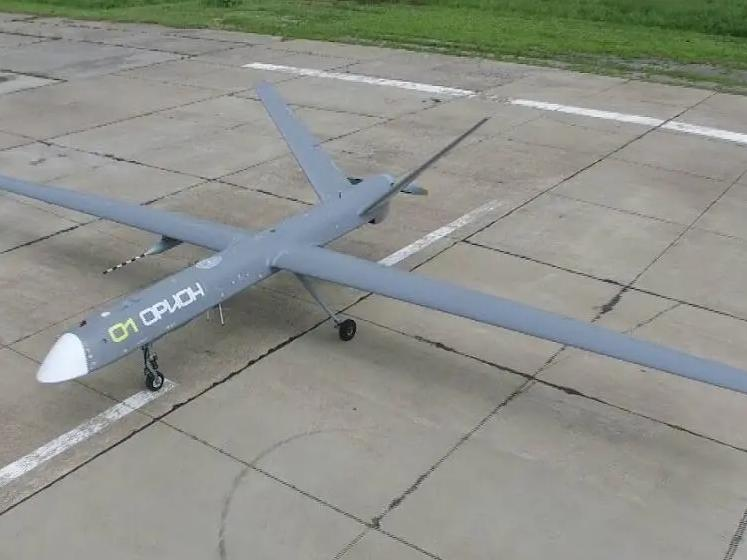
\includegraphics[width=6cm,height=5cm]{Fig/Orion.jpg}
		\caption{\label{Orion}猎户座固定翼无人机}
	\end{minipage}%
	\begin{minipage}[c]{0.5\textwidth}
		\centering
		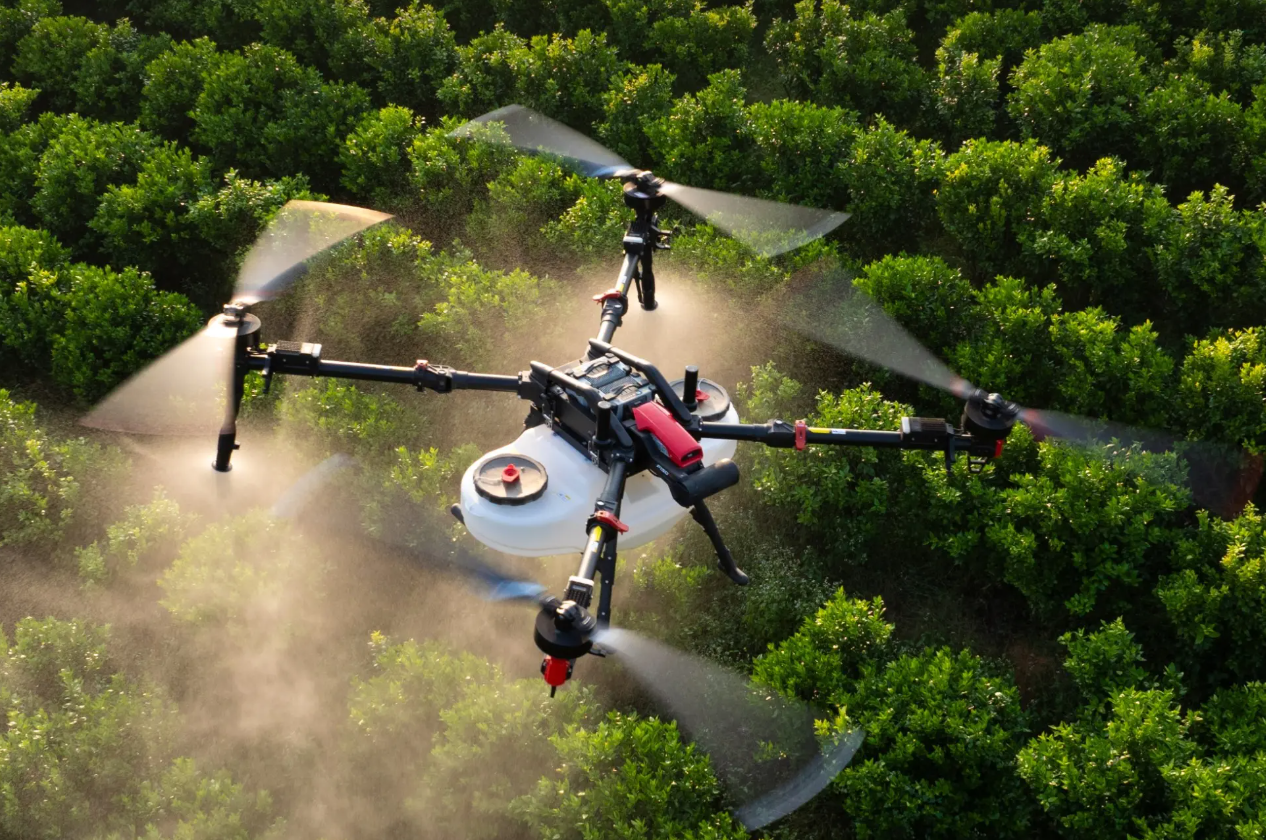
\includegraphics[width=6cm,height=5cm]{Fig/P150PRO.png}
		\caption{\label{P150PRO}极飞P150PRO农业无人机}
	\end{minipage}
\end{figure}

无人机发展百年,种类繁多,不同的任务需求驱动着创造不同类型的无人机。因此按照无人机的任务能力,可将其分为水平起飞着陆(Horizontal Take-off Landing,HTOL)、垂直起飞着陆(Vertical Take-off Landing,VTOL)、混合模型(倾转翼、倾转旋翼和涵道风扇)、直升机和非常规类型\cite{hassanalianClassificationsApplicationsDesign2017}。其中,涵道风扇无人机(Ducted Fan UAV,DFUAV)是指其螺旋桨被封闭在涵道内部的无人机,这些螺旋桨也被称为“风扇”,同时下方安装有若干控制舵面进行控制。DFUAV既有旋翼无人机般的垂直起降能力,又可以像固定翼无人机那样高速巡航,而且这种特殊的配置结构具有空气动力效率高和操作安全性的优势\cite{johnsonModelingControlFlight2006b,zhangReviewDuctedFans2020b,qianImprovingPerformanceDucted2022}。但不如人意的是,与开放旋翼相比,涵道风扇的罩状旋翼在飞行器周围的流场中会表现出强烈的耦合效应\cite{iiiNondimensionalModelingDuctedFan2012},并且由于其特殊的气动布局,DFUAV在垂直起降和水平巡航这两种不同的飞行模式下气动特性也完全不同\cite{johnsonModelingControlFlight2006b},这都对DFUAV的控制器设计提出了挑战。此外,针对DFUAV的轨迹规划的研究相对匮乏,这种研究的不足在一定程度上限制了DFUAV在复杂环境中的高效运作,不利于DFUAV的进一步推广应用。

正因如此,设计出适用于DFUAV的控制策略以及合理的轨迹规划方法,对于DFUAV的进一步发展具有重要意义。

\section{国内外研究现状}

\subsection{涵道风扇无人机}

目前已知的关于涵道风扇无人机的起源最早可以追溯到二十世纪三十年代,由意大利的Stipa和德国的Kort率先在该领域开展研究\cite{iiiNondimensionalModelingDuctedFan2012}。在二十世纪五十年代,美国宇航局在自研Doak VZ-4和Bell X-22涵道风扇垂直起降飞行器时投入了大量精力后取得一些进展,然而他们也发现了一些意料之外的特性,如从悬停到前飞过度时,会出现机头上仰的趋势\cite{cookSummaryLiftLift1993}。Pereira等人\cite{pereiraHoverWindtunnelTesting2008}已经对涵道风扇早期的研究进行了详尽的回顾。

近年来,


这里主要是想推荐一种“学术生态”,即利用各种工具展开科研工作,以达到事半功倍的效果。需要用到以下软件:
\begin{enumerate}[topsep = 0 pt, itemsep= 0 pt, parsep=0pt, partopsep=0pt, leftmargin=44pt, itemindent=0pt, labelsep=6pt, label=(\arabic*)]
	\item 	参考文献管理软件zotero\cite{_m}。很多人使用过endnote,但其实zotero也非常强大,强烈推荐。可到b站观看Struggle with Me出品的视频教程\cite{_k}入门(或其他最新教程,刚开始不推荐使用插件,会增加学习难度)。zotero自带pdf阅读器,也可以设置为使用其他阅读器。在zotero可以打开文件所在位置,故不推荐更改zotero的文件系统(尤其不推荐使用zotfile插件,事实上各种五花八门的插件增加了复杂性,实际上没有带来太多便利性)。理论上只需要包含文献元数据信息的bib文件(可以手动一篇一篇文章地收集)即可使用此模板,因此模板不依赖于任何参考文献管理软件,endnote用户或不使用参考文献管理软件的用户可以忽略本文zotero部分的讲解。
	\item	可截图获取文献中公式的软件mathpix\cite{_h}。在阅读别人的论文时,很可能需要把文章中的公式抄下来放到自己的笔记中,方便以后组会报告甚至论文中使用,这时使用mathpix可直接截图获取\LaTeX{}源码,非常方便。该软件普通邮箱注册可每月50次免费,学校邮箱可100次,若信用卡注册可1000次(最新情况是只能500次了,还要收费20美元,世界变化太快了)。注:随着mathpix的使用成本越来越高,免费次数越来越少,2023起已经不再推荐。目前开源/免费的替代工具为:。\href{https://www.simpletex.cn/}{SimpleTex}和\href{https://p2t.breezedeus.com/}{Pix2Tex}。目前SimpleTex性能比较好,免费但不开源,不排除未来收费的可能
	\item	TeXlive202x、TeXstudio,相当于开发环境和IDE。本模板是基于TeX的发行版TeXlive202x和编辑器TeXstudio进行的,百度这两个关键字分别安装。关于TeXstudio的使用(快捷键等)可另行查找资料。模板还支持更多ide,更多编译方式见GitHub首页readme.md。若在其他窗口打开了编译生成的pdf文件,记得关掉再编译,否则报错。TeXstudio的设置见第二章。
\end{enumerate}

本文的章节安排如下:

第一章,绪论。

第二章,模板简介。主要介绍各文件的内容。

第三章,常用环境。介绍论文写作中常用的环境,包括:图、表、公式、定理。基本涵盖了常用的命令。

%第三章,参考文献设置。本模板对旧版的改动主要是参考文献部分,本章将简单参考文献设置以及
%编译选项的设置等等。


